\documentclass{article}
\usepackage{graphicx}
\usepackage[margin=1.5cm]{geometry}
\usepackage{amsmath}

\begin{document}
\twocolumn

\title{Monday Warm Up: Ohm's Law, Energy and Power in DC Circuits.}
\author{Prof. Jordan C. Hanson}

\maketitle

\section{Memory Bank}

\begin{itemize}
\item $I = \Delta Q / \Delta t$ ... Definition of current.
\item $\Delta V = I R$ ... Ohm's Law.
\item $R = \rho (L/A)$ ... Resistivity, $\rho$, and resistance, $R$, for a conductor with cross-sectional area $A$ and length $L$.
\item $\rho = \rho_0(1+\alpha \Delta T)$ ... Resistivity depends on changes in temperature.
\item $R = R_0(1+\alpha \Delta T)$ ... Resistance depends on changes in temperature.
\item $P = \Delta E/\Delta t$ ... Power is energy or work per unit time.
\item $P = I^2 R = V^2/R = IV$ ... Formulae for power consumption in a DC circuit.
\end{itemize}

\section{Ohm's Law}

\begin{enumerate}
\item What current flows through the bulb of a 3.00-V flashlight when its hot resistance is 3.60 $\Omega$? \\ \vspace{1.5cm}
\item What is the effective resistance of a car’s starter motor when 150 A flows through it as the car battery applies 11.0 V to the motor? \\ \vspace{1.5cm}
\end{enumerate}

\section{Electric Power and Energy}

\begin{enumerate}
\item A charge of 4.00 C passes through a pocket calculator's solar cells in 4.00 h. What is the power output, given the calculator’s voltage output is 3.00 V? \\ \vspace{2cm}
\item (a) Verify that the units of a volt-ampere are watts, as implied by the equation $P=IV$. (b) Show that the units V$^2/\Omega=1$ W, as implied by the equation $P = V^2/R$. (c) Show that the units A$^2 \Omega=1$ W, as implied by the equation $P = I^2 R$. \\ \vspace{3cm}
\item Verify the energy unit equivalence that 1 kW hr $= 3.60\times 10^6$ J. \\ \vspace{2cm}
\item An electric water heater consumes 5.00 kW for 2.00 h per day. What is the cost of running it for one year if electricity costs 12.0 cents per kiloWatt hour? \\ \vspace{2cm}
\item Consider Fig. \ref{fig:1}.  (a) Let $V_0 = 120$ Volts, and $I_0 = 50$ mA.  What is the average power? (b) Let $T = 16.7$ ms be the \textit{period} of the wave, the time between peaks in voltage.  What is $f = 1/T$, the \textit{frequency} of the wave?
\end{enumerate}

\begin{figure}
\centering
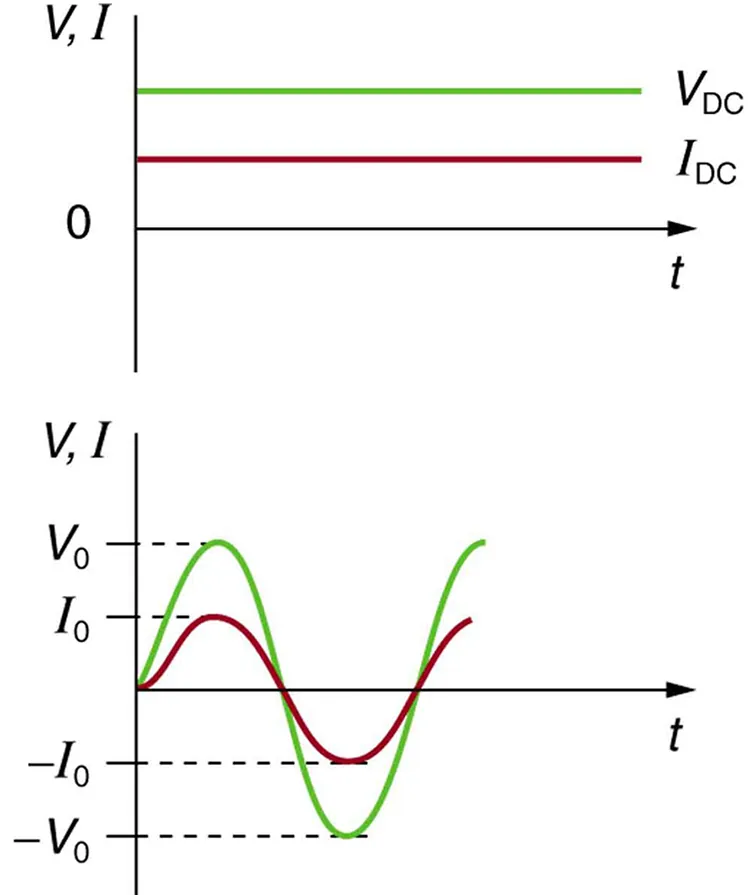
\includegraphics[width=0.24\textwidth,trim=0cm 0cm 0cm 13.5cm,clip=true]{figures/AC_1.png} 
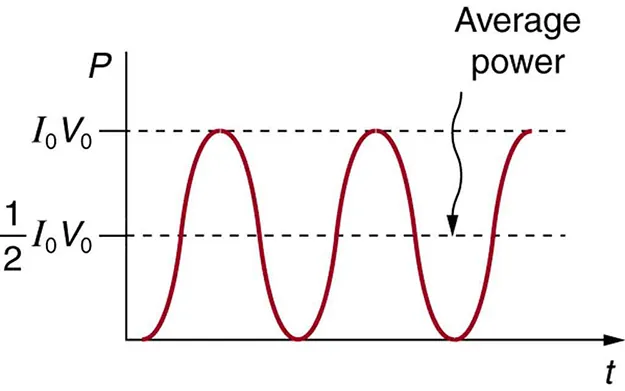
\includegraphics[width=0.24\textwidth]{figures/AC_3.png}
\caption{\label{fig:1} (Left) Voltage and current vs. time in an AC circuit. (Right) Average power in AC circuit.}
\end{figure}

\end{document}
